\documentclass[12pt, a4paper]{article}
\usepackage[utf8]{inputenc}
\usepackage[russian]{babel}
\usepackage[pdftex]{graphicx, color}
\usepackage[left=2cm,right=2cm,top=1.5cm,bottom=2cm]{geometry}
\usepackage{indentfirst}
\usepackage{hyperref}
\usepackage[justification=centering,labelfont=bf]{caption, subcaption}
\usepackage{amsmath, amsfonts, amssymb, amsthm, amsbsy, mathtools}
\usepackage{mdframed}
\usepackage{setspace}
\usepackage{enumitem}
\usepackage[table,xcdraw]{xcolor}
\usepackage{multirow}
\usepackage{float}

% \usepackage{minted}
% \usemintedstyle{tango}
% \renewcommand{\listingscaption}{Листинг}

\onehalfspacing

\title{
    
\includegraphics[height=3cm]{pics/msu.png} \\
    \normalsize{
        Отчёт по практическому заданию по курсу \\
        <<Суперкомпьютерное моделирование и технологии программирования>> \\
    }
    \large{
        \textbf{<<Метод конечных разностей приближенного решения задачи Дирихле для уравнения Пуассона в прямоугольной области>>}\\
        Вариант 35
    }
}
\author{
    \normalsize{Аят Оспанов} \\
    \normalsize{617 группа, ММП, ВМК МГУ, Москва}
}
\date{\normalsize{28 ноября 2017 г.}}

\begin{document}
    \maketitle
    \tableofcontents

    \section{Формулировка задания}
        Требуется методом конечных разностей приближенно решить задачу Дирихле для
        уравнения Пуассона в прямоугольной области. Задание необходимо выполнить на
        следующих ПВС Московского университета:
        \begin{itemize}[leftmargin=1.5cm]
            \item IBM Blue Gene/P
            \item «Ломоносов»
        \end{itemize}

        \subsection{Математическая постановка дифференциальной задачи}
            В прямоугольной области
                $$\Pi = [A_1, A_2] \times [B_1, B_2]$$
            требуется найти дважды гладкую функцию $u = u(x, y)$, удовлетворяющую
            дифференциальному уравнению
            \begin{gather}
                -\Delta u = F(x, y), \quad A_1 < x < A_2, \quad B_1 < y < B_2
                \label{eq:1}
            \end{gather}
            и дополнительному условию
            \begin{gather}
                u(x, y) = \varphi(x, y)
                \label{eq:2}
            \end{gather}
            во всех граничных точках $(x, y)$ прямоугольника. Оператор Лапласа $\Delta$
            определен равенством:
                $$\Delta u = \frac{\partial^2 u}{\partial x^2} + \frac{\partial^2 u}{\partial y^2}$$
            Функции $F(x, y), \varphi(x, y)$ указаны в разделе \ref{sec:cond}.

        \subsection{Разностная схема решения задачи}
            В расчетной области $\Pi$ определяется прямоугольная сетка
                $$\bar\omega_h = \{(x_i, y_j), \quad i = 0, 1, \dots, N_1, \quad j = 0, 1, \dots, N_2\},$$
            где $A_1 = x_0 < x_1 < \dots < x_{N_1} = A_2$ -- разбиение отрезка $[A_1, A_2]$ оси $(Ox)$,\\$B_1 = y_0 < y_1 < \dots < y_{N_1} = B_2$ -- разбиение отрезка $[B_1, B_2]$ оси $(Oy)$.

            Через $\omega_h$ обозначим множество внутренних, а через $\gamma_h$ -- множество граничных узлов сетки $\bar\omega_h$. Пусть $h_i^{(1)} = x_{i + 1} - x_i, \quad i = 0, 1, \dots, N_1 - 1, \quad h_j^{(2)} = y_{j + 1} - y_j, \quad j = 0, 1, \dots, N_2 - 1, $ -- переменный шаг сетки по оси абсцисс и ординат соответственно. Средние шаги сетки определяются равенствами:
            $$\hbar_i^{(1)} = 0.5\big(h_i^{(1)} + h_{i-1}^{(1)}\big), \hbar_j^{(2)} = 0.5\big(h_j^{(2)} + h_{j-1}^{(2)}\big).$$

            Рассмотрим линейное пространство $H$ функций, заданных на сетке $\omega_h$. Будем считать, что в пространстве $H$ задано скалярное произведение и евклидова норма
            \begin{gather}
                (u, v) = \sum\limits_{i=1}^{N_1 - 1} \sum\limits_{j=1}^{N_2 - 1} \hbar_i^{(1)} \hbar_j^{(2)} u_{ij} v_{ij}, \quad ||u|| = \sqrt{(u,u)},
                \label{eq:3}
            \end{gather}
            где $u_{ij} = u(x_i, y_j), v_{ij} = v(x_i, y_j)$ -- любые функции из пространства $H$.

            Для аппроксимации уравнения Пуасона~\eqref{eq:1} воспользуемся пятиточечным разностным оператором Лапласа, который во внутренних узлах сетки определяется равенством:
            \begin{gather*}
                -\Delta_h p_{ij} = \frac{1}{\hbar_i^{(1)}} \Bigg(\frac{p_{ij} - p_{i-1 j}}{h_{i-1}^{(1)}} - \frac{p_{i+1 j} - p_{ij}}{h_i^{(1)}}\Bigg) +
                \frac{1}{\hbar_j^{(1)}} \Bigg(\frac{p_{ij} - p_{i j-1}}{h_{j-1}^{(2)}} - \frac{p_{i j+1} - p_{ij}}{h_j^{(2)}}\Bigg)
            \end{gather*}
            Здесь предполагается, что функция $p = p(x_i, y_j)$ определена во всех узлах сетки $\bar\omega_h$.

            Приближенным решением задачи \eqref{eq:1}, \eqref{eq:2} называется функция $p = p(x_i, y_j)$, удовлетворяющая уравнениям
            \begin{gather}
            \begin{cases}
                -\Delta_h p_{ij} = F(x_i, y_j), \quad (x_i, y_j) \in \omega_h,\\
                p_{ij} = \varphi(x_i, y_j), \quad (x_i, y_j) \in \gamma_h.
            \end{cases}
            \label{eq:4}
            \end{gather}

            Эти соотношения представляют собой систему линейных алгебраических уравнений с числом уравнений равным числу неизвестных и определяют единственным образом неизвестные значения $p_{ij}$. Совокупность уравнений \eqref{eq:4} называется разностной схемой для задачи \eqref{eq:1}, \eqref{eq:2}.

        \subsection{Метод решения системы линейных алгебраических уравнений}
            Приближенное решение системы уравнений \eqref{eq:4} может быть получено итерационным методом сопряженных градиентов. В этом методе начальное приближение
                \begin{gather*}
                \begin{cases}
                    p_{ij}^{(0)} &= \varphi(x_i, y_j), \quad (x_i, y_j) \in \gamma_h,\\
                    p_{ij}^{(0)} &= \text{любые числа}, \quad (x_i, y_j) \in \omega_h,
                \end{cases}
                \end{gather*}

            Последующие итерации осуществляются по формулам:
                $$p_{ij}^{(k+1)} = p_{ij}^{(k)} - \tau_{k+1} g_{ij}^{(k)}, \quad k=0,1,2,\dots$$
            Здесь
                $$\tau_{k+1} = \frac{(r^{(k)},g^{(k)})}{(-\Delta_h g^{(k)},g^{(k)})},$$
            градиент
                \begin{gather*}
                \begin{cases}
                    g_{ij}^{(k)} &= r_{ij}^{(k)} - \alpha_k g_{ij}^{(k - 1)}, \quad k=1,2,\dots,\\
                    g_{ij}^{(0)} &= r_{ij}^{(0)},
                \end{cases}
                \end{gather*}
            коэффициент
                $$\alpha_{k} = \frac{(-\Delta_h r^{(k)},g^{(k-1)})}{(-\Delta_h g^{(k-1)},g^{(k-1)})},$$
            невязка
                \begin{gather*}
                \begin{cases}
                    r_{ij}^{(k)} &= -\Delta_h p_{ij}^{(k)} - F(x_i, y_j), \quad (x_i, y_j) \in \omega_h\\
                    r_{ij}^{(k)} &= 0, \quad (x_i, y_j) \in \gamma_h
                \end{cases}
                \end{gather*}

            Итерационный процесс останавливается, как только
            $$||p^{(n)} - p^{(n-1)}|| < \varepsilon,$$
            где $\varepsilon$ -- заранее выбранное положительное число.

    \section{Условия задания}\label{sec:cond}
        В данном варианте (вариант 35) правая часть уравнения \eqref{eq:1} и граничное условие \eqref{eq:2} определяются следующим образом:
            \begin{gather}
                F(x, y) = \frac{8(1 - x^2 - y^2)}{(1 + x^2 + y^2)^3} \label{eq:F}\\
                \varphi(x, y) = \frac{2}{1 + x^2 + y^2} \label{eq:phi}
            \end{gather}

        Дифференциальную задачу надо решить для данных функций на прямоугольнике $$\Pi = [0, 2] \times [0, 2]$$ на неравномерной сетке, определенной равенствами:
            \begin{gather}
            \begin{aligned}
                x_i &= A_2 f(i / N_1) + A_1 (1 - f(i / N_1)), \quad i = 0, 1, \dots, N_1,\\
                y_j &= B_2 f(j / N_2) + B_1 (1 - f(j / N_2)), \quad j = 0, 1, \dots, N_2.\\
            \end{aligned}
            \end{gather}
        где
            $$f(t) = \frac{(1 + t)^q - 1}{2^q - 1}, \quad 0 \leq t \leq 1, \quad q = 3/2$$

    \section{Аналитическое решение}
        Для решения задачи \eqref{eq:1} с граничными условиями \eqref{eq:2}, предположим, что $u(x, y) = \varphi(x, y)$ для всех точек прямоугольника. Тогда должно выполнятся
        $$-\Delta \varphi(x, y) = F(x, y)$$

        Проверим это: т.к. $\varphi(x, y)$ симметрична относительно $x$ и $y$, то просто найдем $\frac{\partial^2 \varphi(x, y)}{\partial x^2}$:
        \begin{gather*}
        \begin{aligned}
            \frac{\partial^2 \varphi(x, y)}{\partial x^2} &= \frac{\partial}{\partial x} \frac{\partial \varphi(x, y)}{\partial x} = \Big\{
                \frac{\partial}{\partial x} \varphi(x, y) = \frac{\partial}{\partial x} \frac{2}{1 + x^2 + y^2} = \frac{-4x}{(1 + x^2 + y^2)^2}
            \Big\} =\\
            &= \frac{\partial}{\partial x} \frac{-4x}{(1 + x^2 + y^2)^2} = \frac{16x^2 - 4(1 + x^2 + y^2)}{(1 + x^2 + y^2)^3} = \frac{12x^2 - 4y^2 - 4}{(1 + x^2 + y^2)^3}
        \end{aligned}
        \end{gather*}

        Теперь посчитаем $-\Delta \varphi(x, y)$:
        \begin{gather*}
        \begin{aligned}
            -\Delta \varphi(x, y) &= -\frac{12x^2 - 4y^2 - 4}{(1 + x^2 + y^2)^3} - \frac{12y^2 - 4x^2 - 4}{(1 + x^2 + y^2)^3} = \\
            &= -\frac{12x^2 - 4y^2 - 4 + 12y^2 - 4x^2 - 4}{(1 + x^2 + y^2)^3} = -\frac{8x^2 + 8y^2 - 8}{(1 + x^2 + y^2)^3} = \\
            &= \frac{8(1 - x^2 - y^2)}{(1 + x^2 + y^2)^3} = F(x, y)
        \end{aligned}
        \end{gather*}

        Т.к. решение задачи Дирихле единственное, то получаем, что наше предположение верно и $$u(x, y) = \frac{2}{1 + x^2 + y^2}$$ на всем прямоугольнике.

    \section{Краткое описание проделанной работы}
        Для создания параллельной программы, решающей дифференциальное уравнение, были использованы язык \verb|C++| и библиотеки MPI и OpenMP. Параллелизация MPI выполнялась следующим образом:
        \begin{itemize}[leftmargin=1.5cm]
            \item Сетка разделялась на $2^p$ заданных процессов так, чтобы по оси $Ox$ было $\big[\frac{p}{2}\big]$ блоков, по оси $Oy$ -- $\big(1 - \big[\frac{p}{2}\big]\big)$. Каждому процессу соответствует один блок.
            \item Каждый блок расширялся на 1 строку/столбец влево/вправо для хранения данных соседних строк/столбцов (если таковые есть)
            \item Каждый процесс, после определенных вычислений, обменивался данными с соседними.
        \end{itemize}

        Параллелизация OpenMP проводилась в каждом процессе для распараллеливания циклов при подсчетах.

        Для удобства была использована парадигма ООП:
        \begin{itemize}[leftmargin=1.5cm]
            \item Каждая двумерная функция представлялась как класс Func2D
            \item В классе Func2D были перегружены следующие операторы (приведены основные):
            \begin{itemize}
                \item умножения на класс Func2D -- скалярное произведение
                \item умножения на число
                \item оператор $\sim$ -- оператор Лапласа
            \end{itemize}
            \item Реализован класс-синглтон MPIHelper -- обертка над MPI
            \item Реализован класс ConjugateGradientMethod -- собственно сам метод сопряженных градиентов
        \end{itemize}

        Также предусмотрена возможность включать директивы OpenMP с помощью задания идентификатора \verb|USE_OMP| при компиляции программы (\verb|-D"USE_OMP"|).

    \section{Результаты для <<IBM BlueGene/P>>}
        Написанная программа многократно запускалась с разными параметрами на суперкомпьютере IBM BlueGene/P. Т.к. использовалась неравномерная сетка, то подсчеты проводились относительно долго по сравнению с равномерной сеткой, даже при предварительном подсчете шагов сетки. В связи с этим, на компьютере BlueGene/P на 1 процессоре программа не укладывалась в заданные рамки 2х часов. Поэтому было решено ограничить количество итераций, что не повлияет на подсчет ускорений. По итогу замеров времени работы, получились результаты, представленные в Таблице \ref{tab:bg_mpi500} для версии MPI без использования OpenMP директив и в Таблице \ref{tab:bg_omp500} для версии MPI с OpenMP директивами (3 нити на процесс).

        В дополнение к запускам на 500 итераций, были сделаны замеры времени работы программы до схождения итерационного процесса. Результаты можно посмотреть в Таблицах \ref{tab:bg_mpi_full} и \ref{tab:bg_omp_full} в Разделе ``\nameref{sec:appdx}''.

        \begin{table}[H]
            \centering
            \caption{MPI версия программы на 500 итераций на BlueGene/P}
            \label{tab:bg_mpi500}
            \begin{tabular}{llll}
            \rowcolor[HTML]{C0C0C0}
            \textbf{Число процессоров} & \textbf{Число точек сетки}                   & \textbf{Время решения, сек} & \textbf{Ускорение} \\
            \rowcolor[HTML]{EFEFEF}
            1                          & \multicolumn{1}{c}{\cellcolor[HTML]{EFEFEF}} & 916.56                      & 1                  \\
            64                         &                                              & 14.70                       & 62.35              \\
            128                        &                                              & 7.87                        & 116.46             \\
            256                        &                                              & 4.11                        & 223.01             \\
            512                        & \multirow{-4}{*}{1000 $\times$ 1000}         & 2.34                        & 391.70             \\
            \rowcolor[HTML]{EFEFEF}
            1                          &                                              & 3737.03                     & 1                  \\
            64                         &                                              & 56.71                       & 65.90              \\
            128                        &                                              & 29.12                       & 128.33             \\
            256                        &                                              & 14.75                       & 253.36             \\
            512                        & \multirow{-4}{*}{2000 $\times$ 2000}         & 7.92                        & 471.85
            \end{tabular}
        \end{table}

        \begin{table}[H]
            \centering
            \caption{MPI+OpenMP версия программы на 500 итераций на BlueGene/P}
            \label{tab:bg_omp500}
            \begin{tabular}{llll}
            \rowcolor[HTML]{C0C0C0}
            \textbf{Число процессоров} & \textbf{Число точек сетки}                   & \textbf{Время решения, сек} & \textbf{Ускорение} \\
            \rowcolor[HTML]{EFEFEF}
            1                          & \multicolumn{1}{c}{\cellcolor[HTML]{EFEFEF}} & 321.63                      & 2.85               \\
            64                         &                                              & 5.71                        & 160.52             \\
            128                        &                                              & 3.38                        & 271.17             \\
            256                        &                                              & 2.00                        & 458.28             \\
            512                        & \multirow{-4}{*}{1000 $\times$ 1000}         & 1.32                        & 694.36             \\
            \rowcolor[HTML]{EFEFEF}
            1                          &                                              & 1292.99                     & 2.89               \\
            64                         &                                              & 20.52                       & 182.12             \\
            128                        &                                              & 10.93                       & 341.91             \\
            256                        &                                              & 5.73                        & 652.19             \\
            512                        & \multirow{-4}{*}{2000 $\times$ 2000}         & 3.38                        & 1105.63
            \end{tabular}
        \end{table}

        Также для удобства сравнения MPI и MPI+OpenMP версий программ представлена Таблица \ref{tab:bg_mpi_to_omp_500}.

        \begin{table}[H]
            \centering
            \caption{Сравнение MPI версии программы с MPI+OpenMP версией на BlueGene/P ($S_{MPI}$ -- ускорение MPI версии программы, $S_{MPI+OMP}$ -- ускорение MPI+OpenMP версии программы)}
            \label{tab:bg_mpi_to_omp_500}
            \begin{tabular}{llllc}
            \rowcolor[HTML]{C0C0C0}
            Число процессоров & Число точек сетки                    & $S_{MPI}$ & $S_{MPI+OMP}$ & \multicolumn{1}{l}{\cellcolor[HTML]{C0C0C0}$S_{MPI+OMP}/S_{MPI}$} \\
            \rowcolor[HTML]{EFEFEF}
            1                 &                                      & 1         & 2.85          & 2.85                                                              \\
            64                &                                      & 62.35     & 160.52        & 2.57                                                              \\
            128               &                                      & 116.46    & 271.17        & 2.33                                                              \\
            256               &                                      & 223.01    & 458.28        & 2.05                                                              \\
            512               & \multirow{-4}{*}{1000 $\times$ 1000} & 391.7     & 694.36        & 1.77                                                              \\
            \rowcolor[HTML]{EFEFEF}
            1                 &                                      & 1         & 2.89          & 2.89                                                              \\
            64                &                                      & 65.9      & 182.12        & 2.76                                                              \\
            128               &                                      & 128.33    & 341.91        & 2.66                                                              \\
            256               &                                      & 253.36    & 652.19        & 2.57                                                              \\
            512               & \multirow{-4}{*}{2000 $\times$ 2000} & 471.85    & 1105.63       & 2.34
            \end{tabular}
        \end{table}

        \subsection{Выводы}
            Как видно из Таблицы \ref{tab:bg_mpi500}, ускорение программы линейно относительно количества процессоров. При этом на сетке $1000 \times 1000$ ускорение чуть меньше, чем количество процессоров, тогда как на сетке $2000 \times 2000$ ускорение примерно равно количеству процессоров. Связано это с нагруженностью процессоров. При большой сетке нагруженность больше, что увеличивает производительность. Также из Таблицы \ref{tab:bg_mpi_to_omp_500} видно, что ускорение MPI+OpenMP версии примерно в 3 раза больше, чем у MPI версии, что подтвреждает теоретическое ускорение при использовании трех нитей OpenMP.

    \section{Результаты для <<Ломоносов>>}
        Программа также тестировалась на суперкомпьютере <<Ломоносов>>. Но по сравнению с BlueGene/P, на Ломоносов использовалась только MPI версия. На данном компьютере также ограничивалось количество итераций. В результате запусков получилась Таблица~\ref{tab:lom_mpi500}
        \begin{table}[H]
            \centering
            \caption{MPI версия программы на 500 итераций на Ломоносов}
            \label{tab:lom_mpi500}
            \begin{tabular}{llll}
            \rowcolor[HTML]{C0C0C0}
            \textbf{Число процессоров} & \textbf{Число точек сетки}                   & \textbf{Время решения, сек} & \textbf{Ускорение} \\
            \rowcolor[HTML]{EFEFEF}
            1                 &                                      & 139.68             & 1         \\
            8                 &                                      & 19.48              & 7.17      \\
            16                &                                      & 8.98               & 15.55     \\
            32                &                                      & 4.53               & 30.83     \\
            64                &                                      & 2.79               & 50.06     \\
            128               & \multirow{-5}{*}{1000 $\times$ 1000} & 1.83               & 76.33     \\
            \rowcolor[HTML]{EFEFEF}
            1                 &                                      & 559.45             & 1         \\
            8                 &                                      & 80.42              & 6.96      \\
            16                &                                      & 39.05              & 14.33     \\
            32                &                                      & 19.64              & 28.49     \\
            64                &                                      & 9.58               & 58.4      \\
            128               & \multirow{-5}{*}{2000 $\times$ 2000} & 4.85               & 115.35
            \end{tabular}
        \end{table}

        Также, как и в случае с BlueGene/P, для Ломоносов можно посмотреть результаты работы программы до схождения в Таблице \ref{tab:lom_mpi_full} в Разделе ``\nameref{sec:appdx}''.

        \subsection{Выводы}
            По таблице \ref{tab:lom_mpi500} можно сделать следующие выводы: для сетки $1000 \times 1000$ ускорение больше для меньших количеств процессоров, а именно для 8, 16 и 32, в то время как для сетки $2000 \times 2000$ ускорение больше для 64 и 128 процессоров. Объяснить это можно нагруженностью процессоров и объемом обмениваемых процессами данных. Если в случае малых количеств процессоров и малой сетки процессоры нагружаются достаточно, то при большой сетке процессоры делают больше вычислений и процессы обмениваются большим количеством данных (т.к. данные делятся на меньшее количество процессов), что увеличивает время работы программы. Данного являения на суперкомпьютере BlueGene/P не наблюдалось, т.к. там используются от 64 процессоров. В случае от 64 процессоров, на Ломоносов та же ситуация, что и с BlueGene/P: ускорение больше для большей сетки, т.к. объем обмениваемых данных меньше.

    \section{Результаты численного решения задачи}
        В итоге работы программы, были получены решения с указанными в Таблице \ref{tab:res} невязками между численным и аналитическим решениями и количеством итераций до схождения.
        \begin{table}[H]
            \centering
            \caption{Замеры для численного метода}
            \label{tab:res}
            \begin{tabular}{|l|l|l|}
            \hline
            \textbf{Размер сетки} & \textbf{Невязка} & \textbf{Количество итераций} \\ \hline
            $1000 \times 1000$    & 0.010209         & 1693                         \\ \hline
            $2000 \times 2000$    & 0.020420         & 3251                         \\ \hline
            \end{tabular}
        \end{table}

        Ниже представлены графики решений дифференицальной задачи на сетке $2000 \times 2000$. По графикам разницы между численным решением (Рис. \ref{fig:plot_a}) и аналитическим решением (Рис. \ref{fig:plot_b}) не видно, т.к. погрешность в каждой точке относительно мала, что видно из Рис. \ref{fig:plot_diff_b}. На Рис. \ref{fig:plot_diff_a} можно увидеть график погрешности в увеличенном масштабе.
        \begin{figure}[H]
            \centering
            \begin{subfigure}[b]{0.49\textwidth}
                \centering
                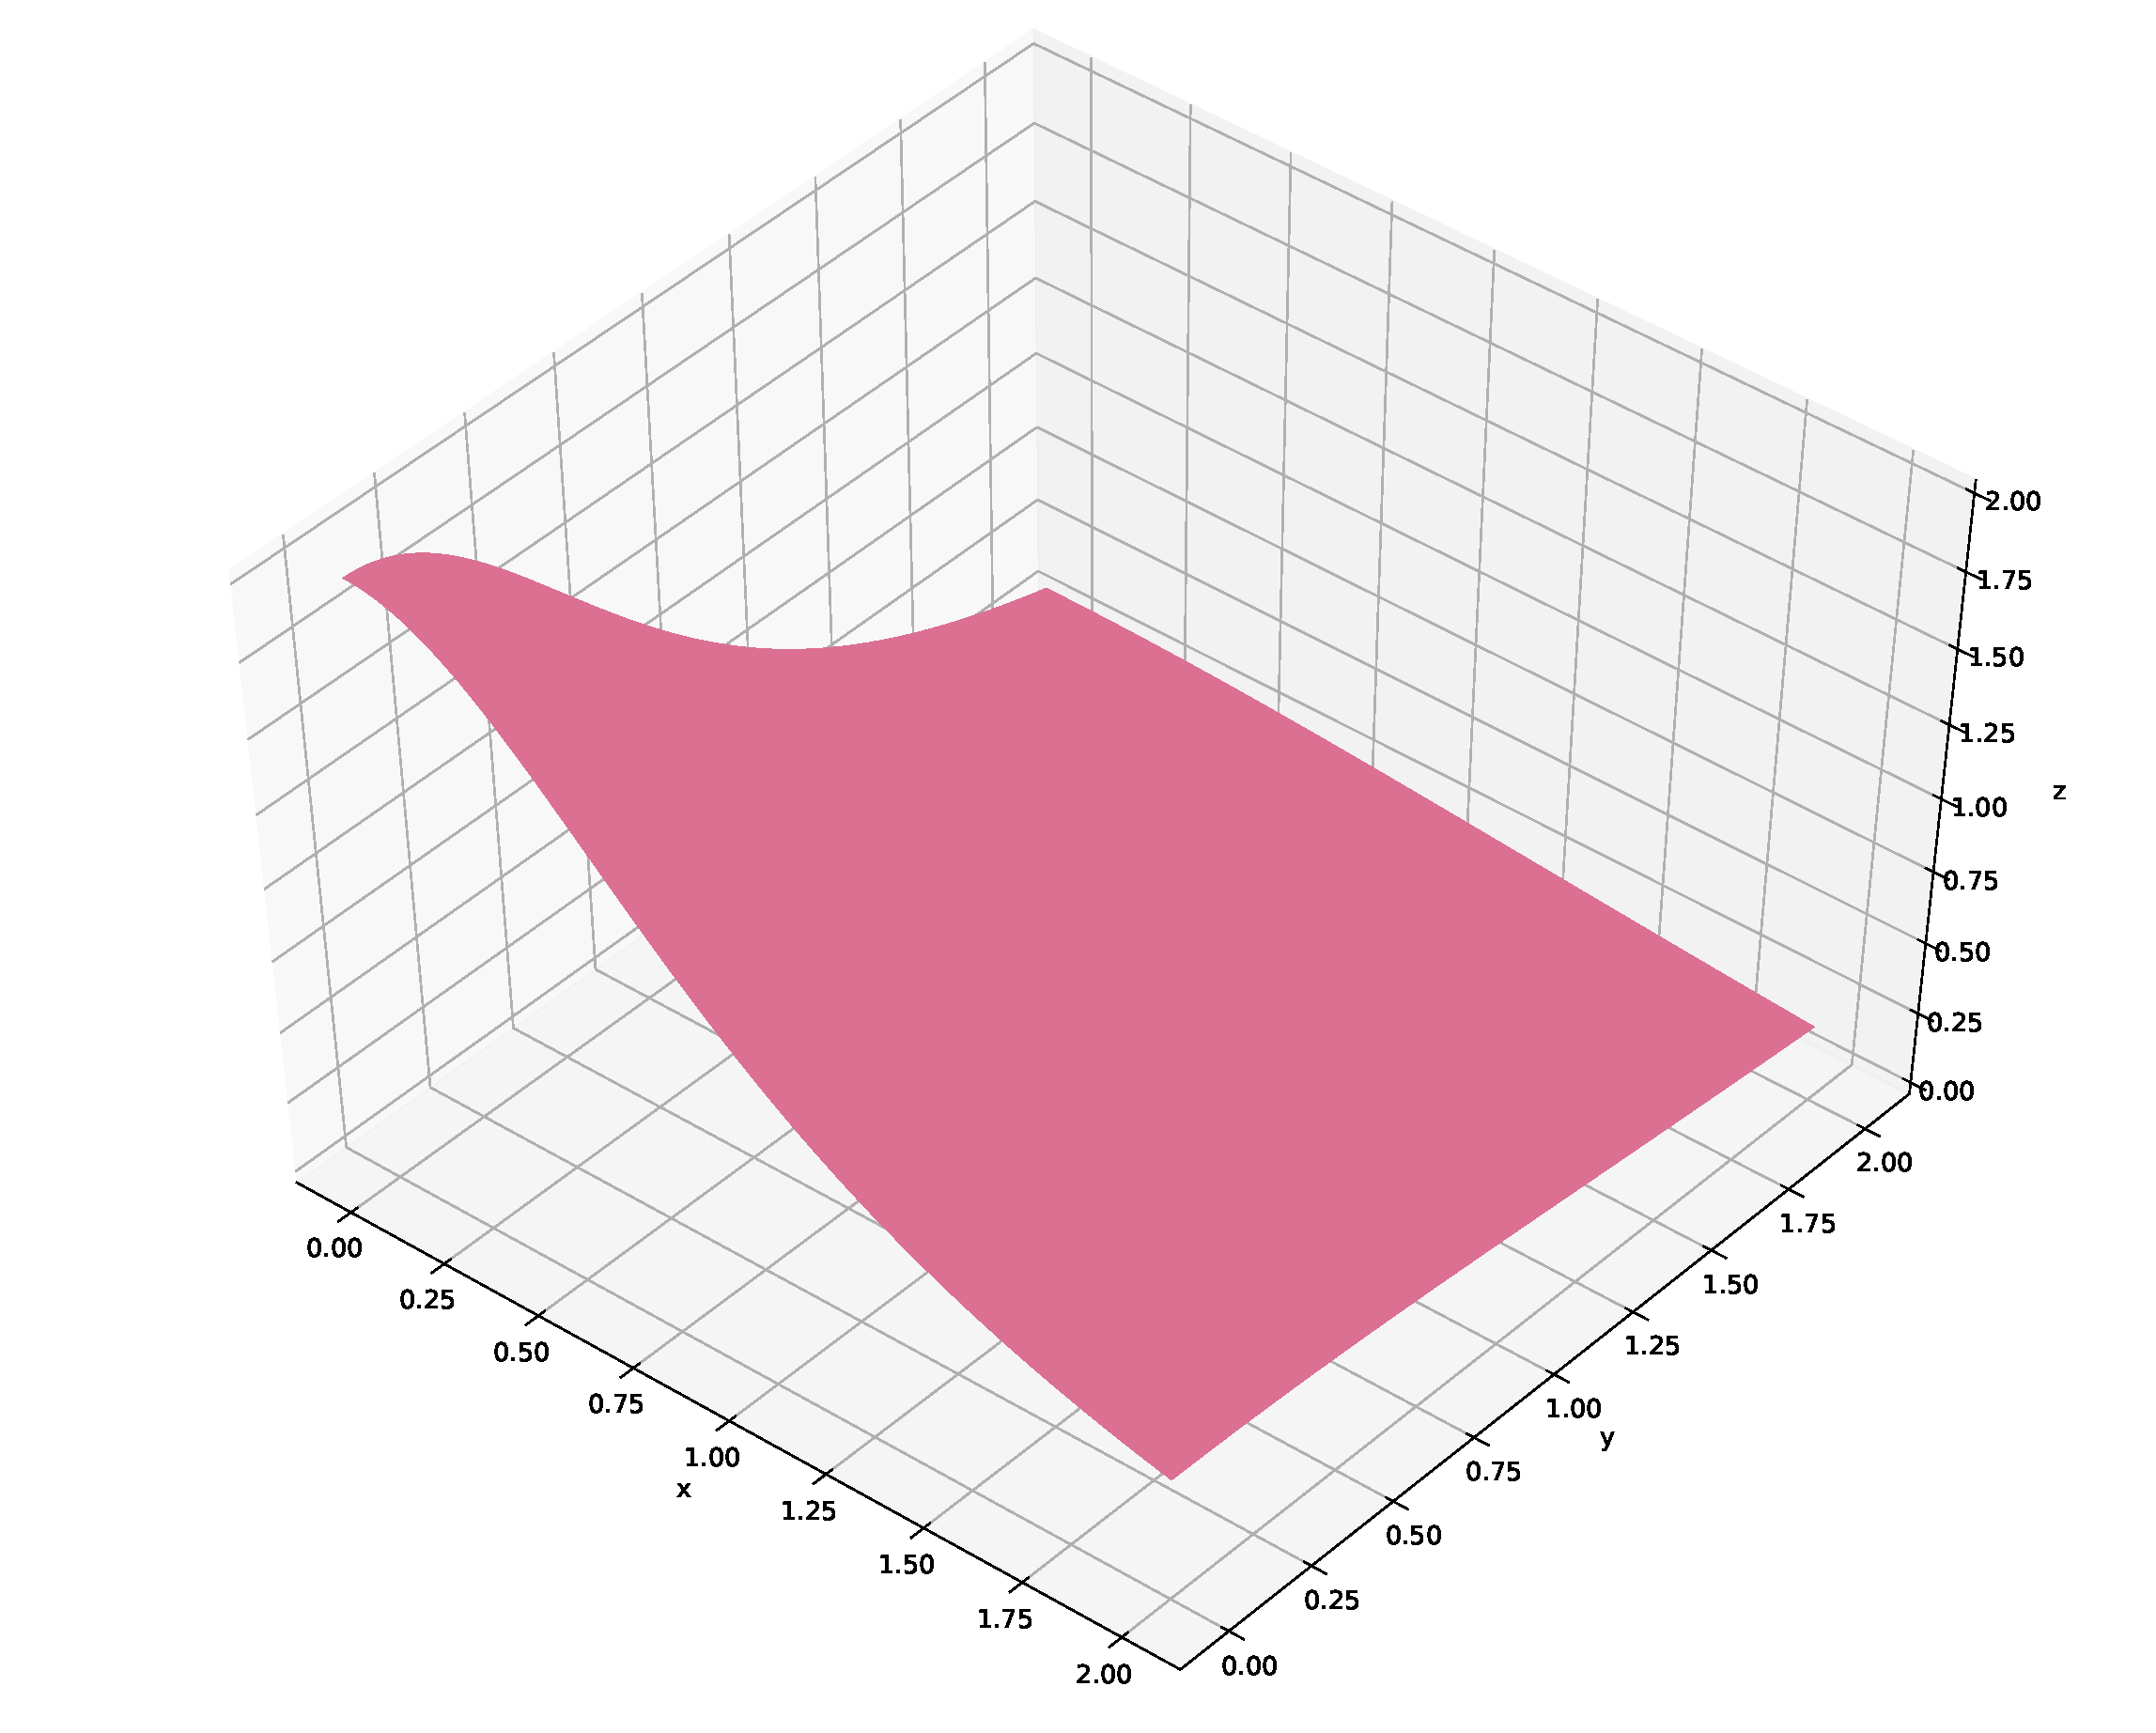
\includegraphics[width=\textwidth]{pics/cg.pdf}
                \caption{Численное решение}
                \label{fig:plot_a}
            \end{subfigure}
            \begin{subfigure}[b]{0.49\textwidth}
                \centering
                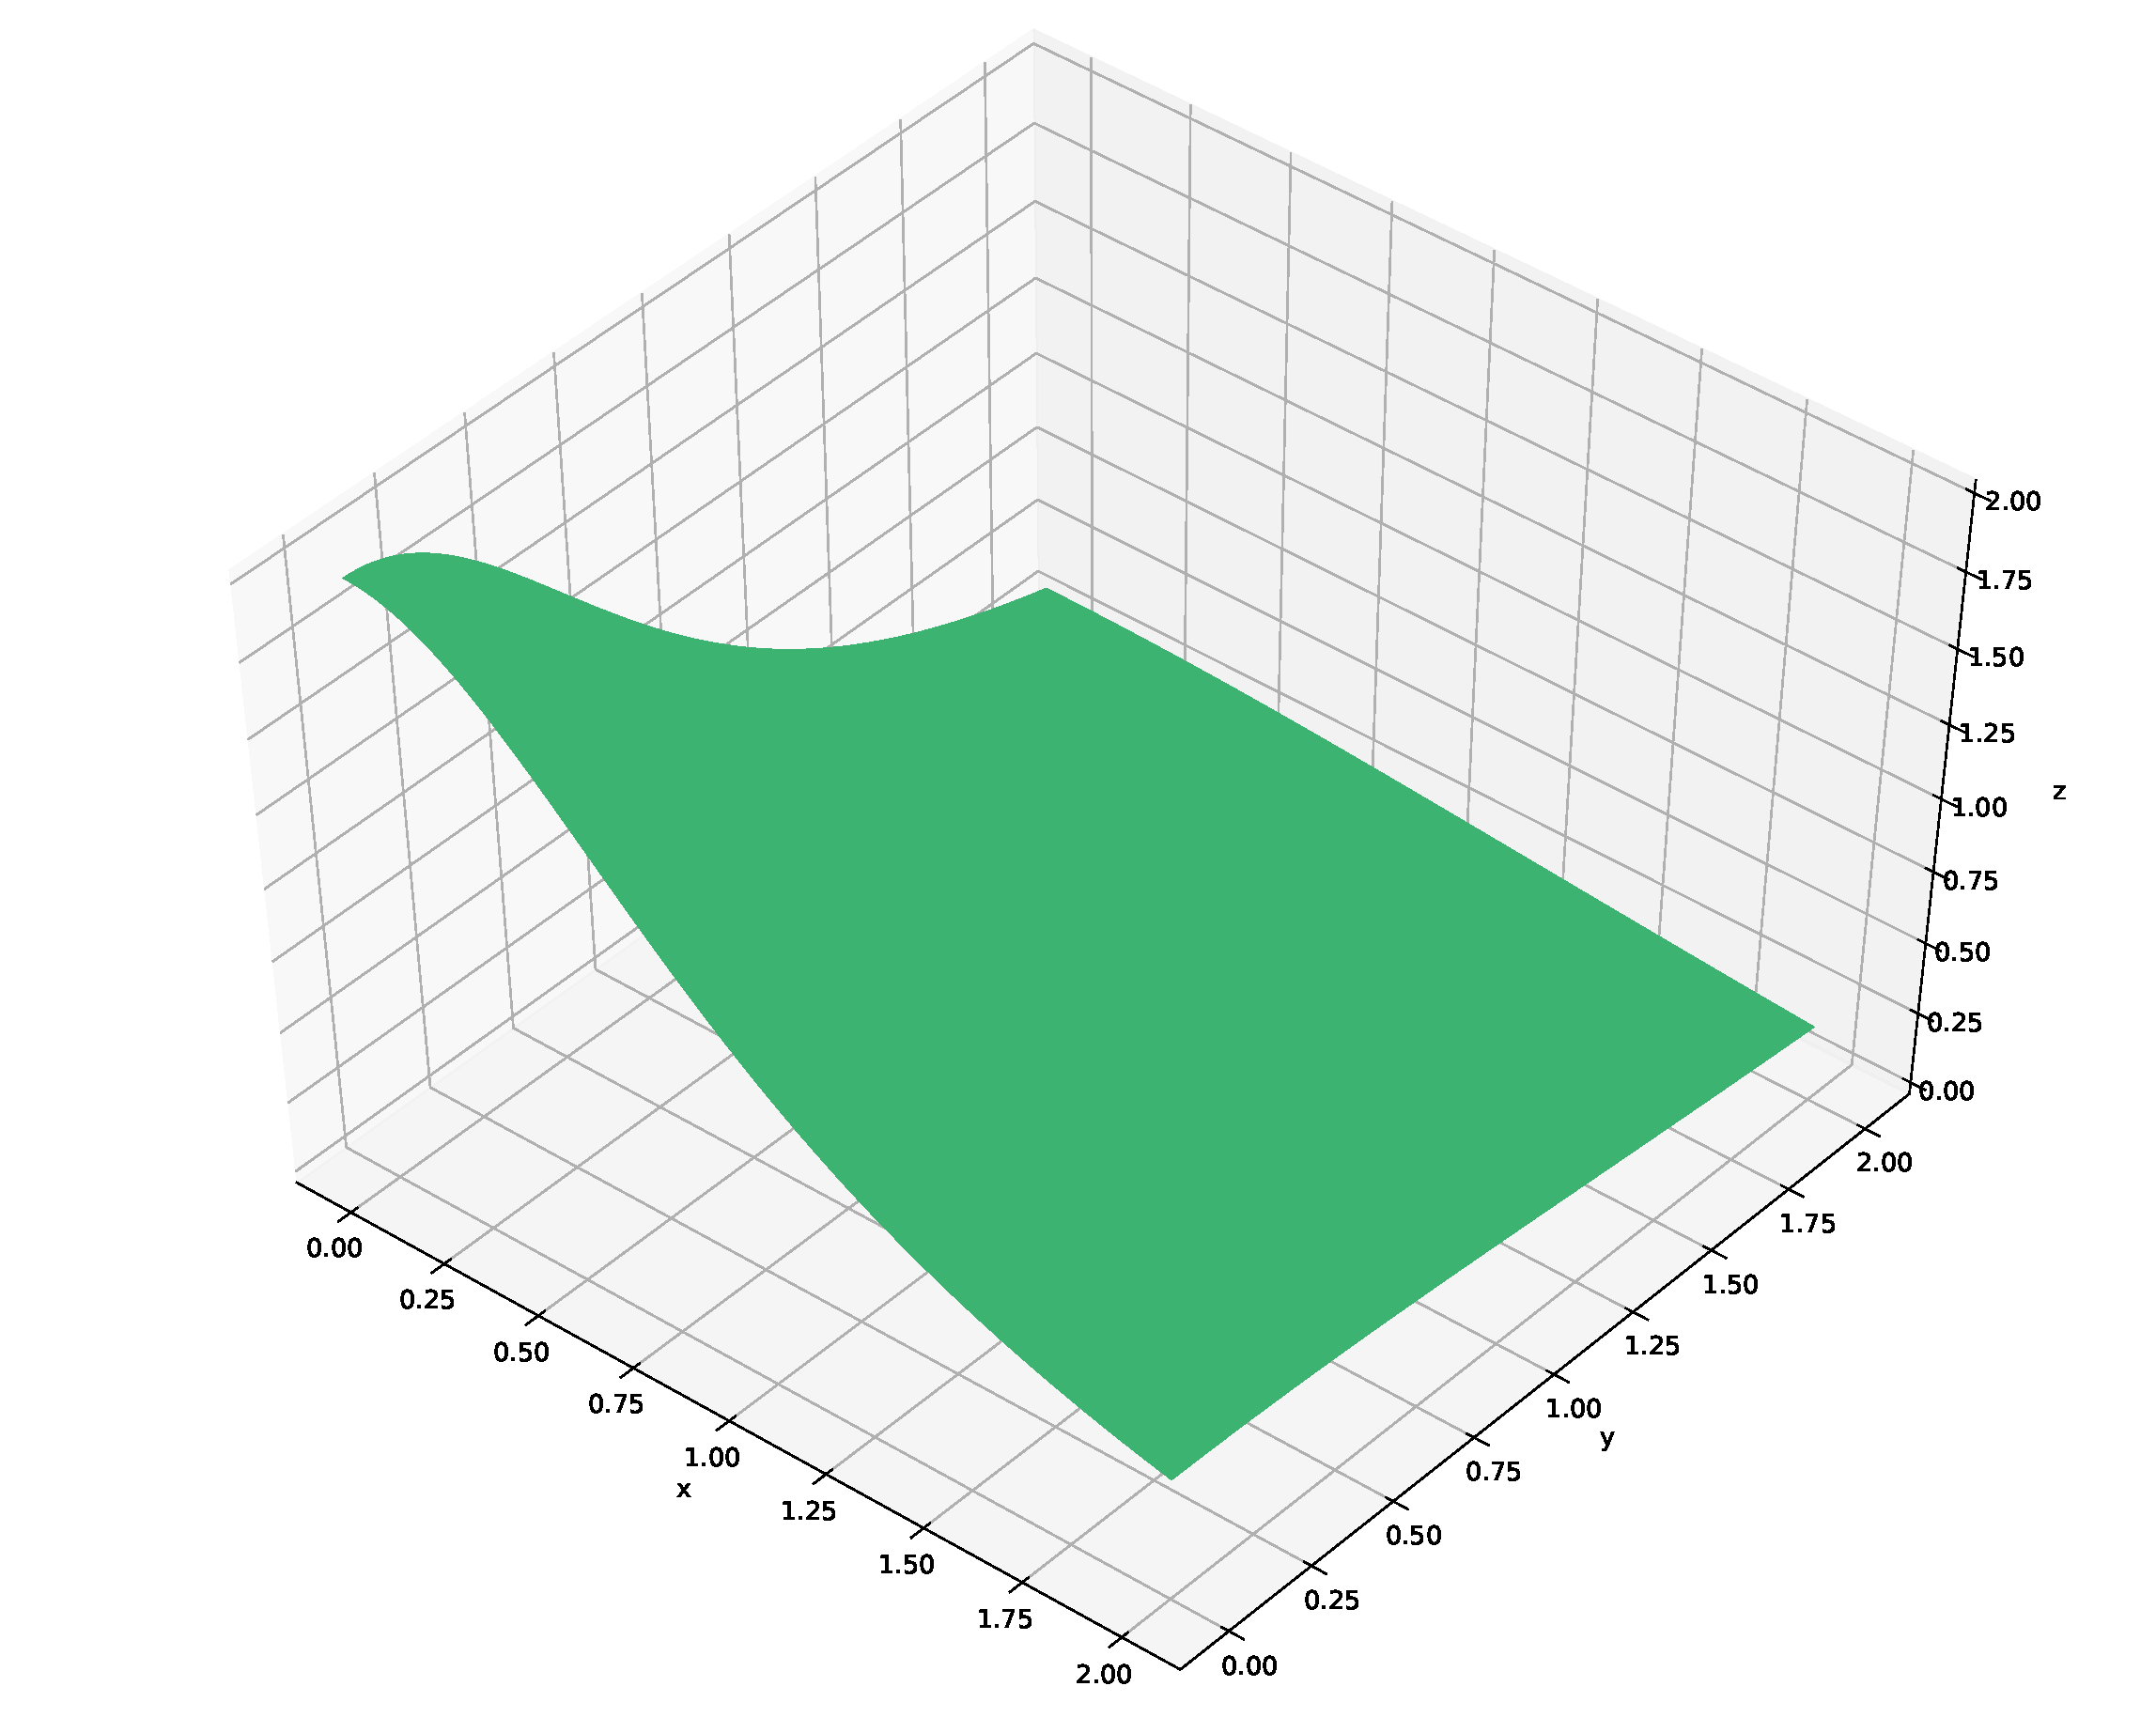
\includegraphics[width=\textwidth]{pics/real.pdf}
                \caption{Аналитическое решение}
                \label{fig:plot_b}
            \end{subfigure}
            \caption{Графики решения дифференицальной задачи}
            \label{fig:plot}
        \end{figure}

        \begin{figure}[H]
            \centering
            \begin{subfigure}[b]{0.49\textwidth}
                \centering
                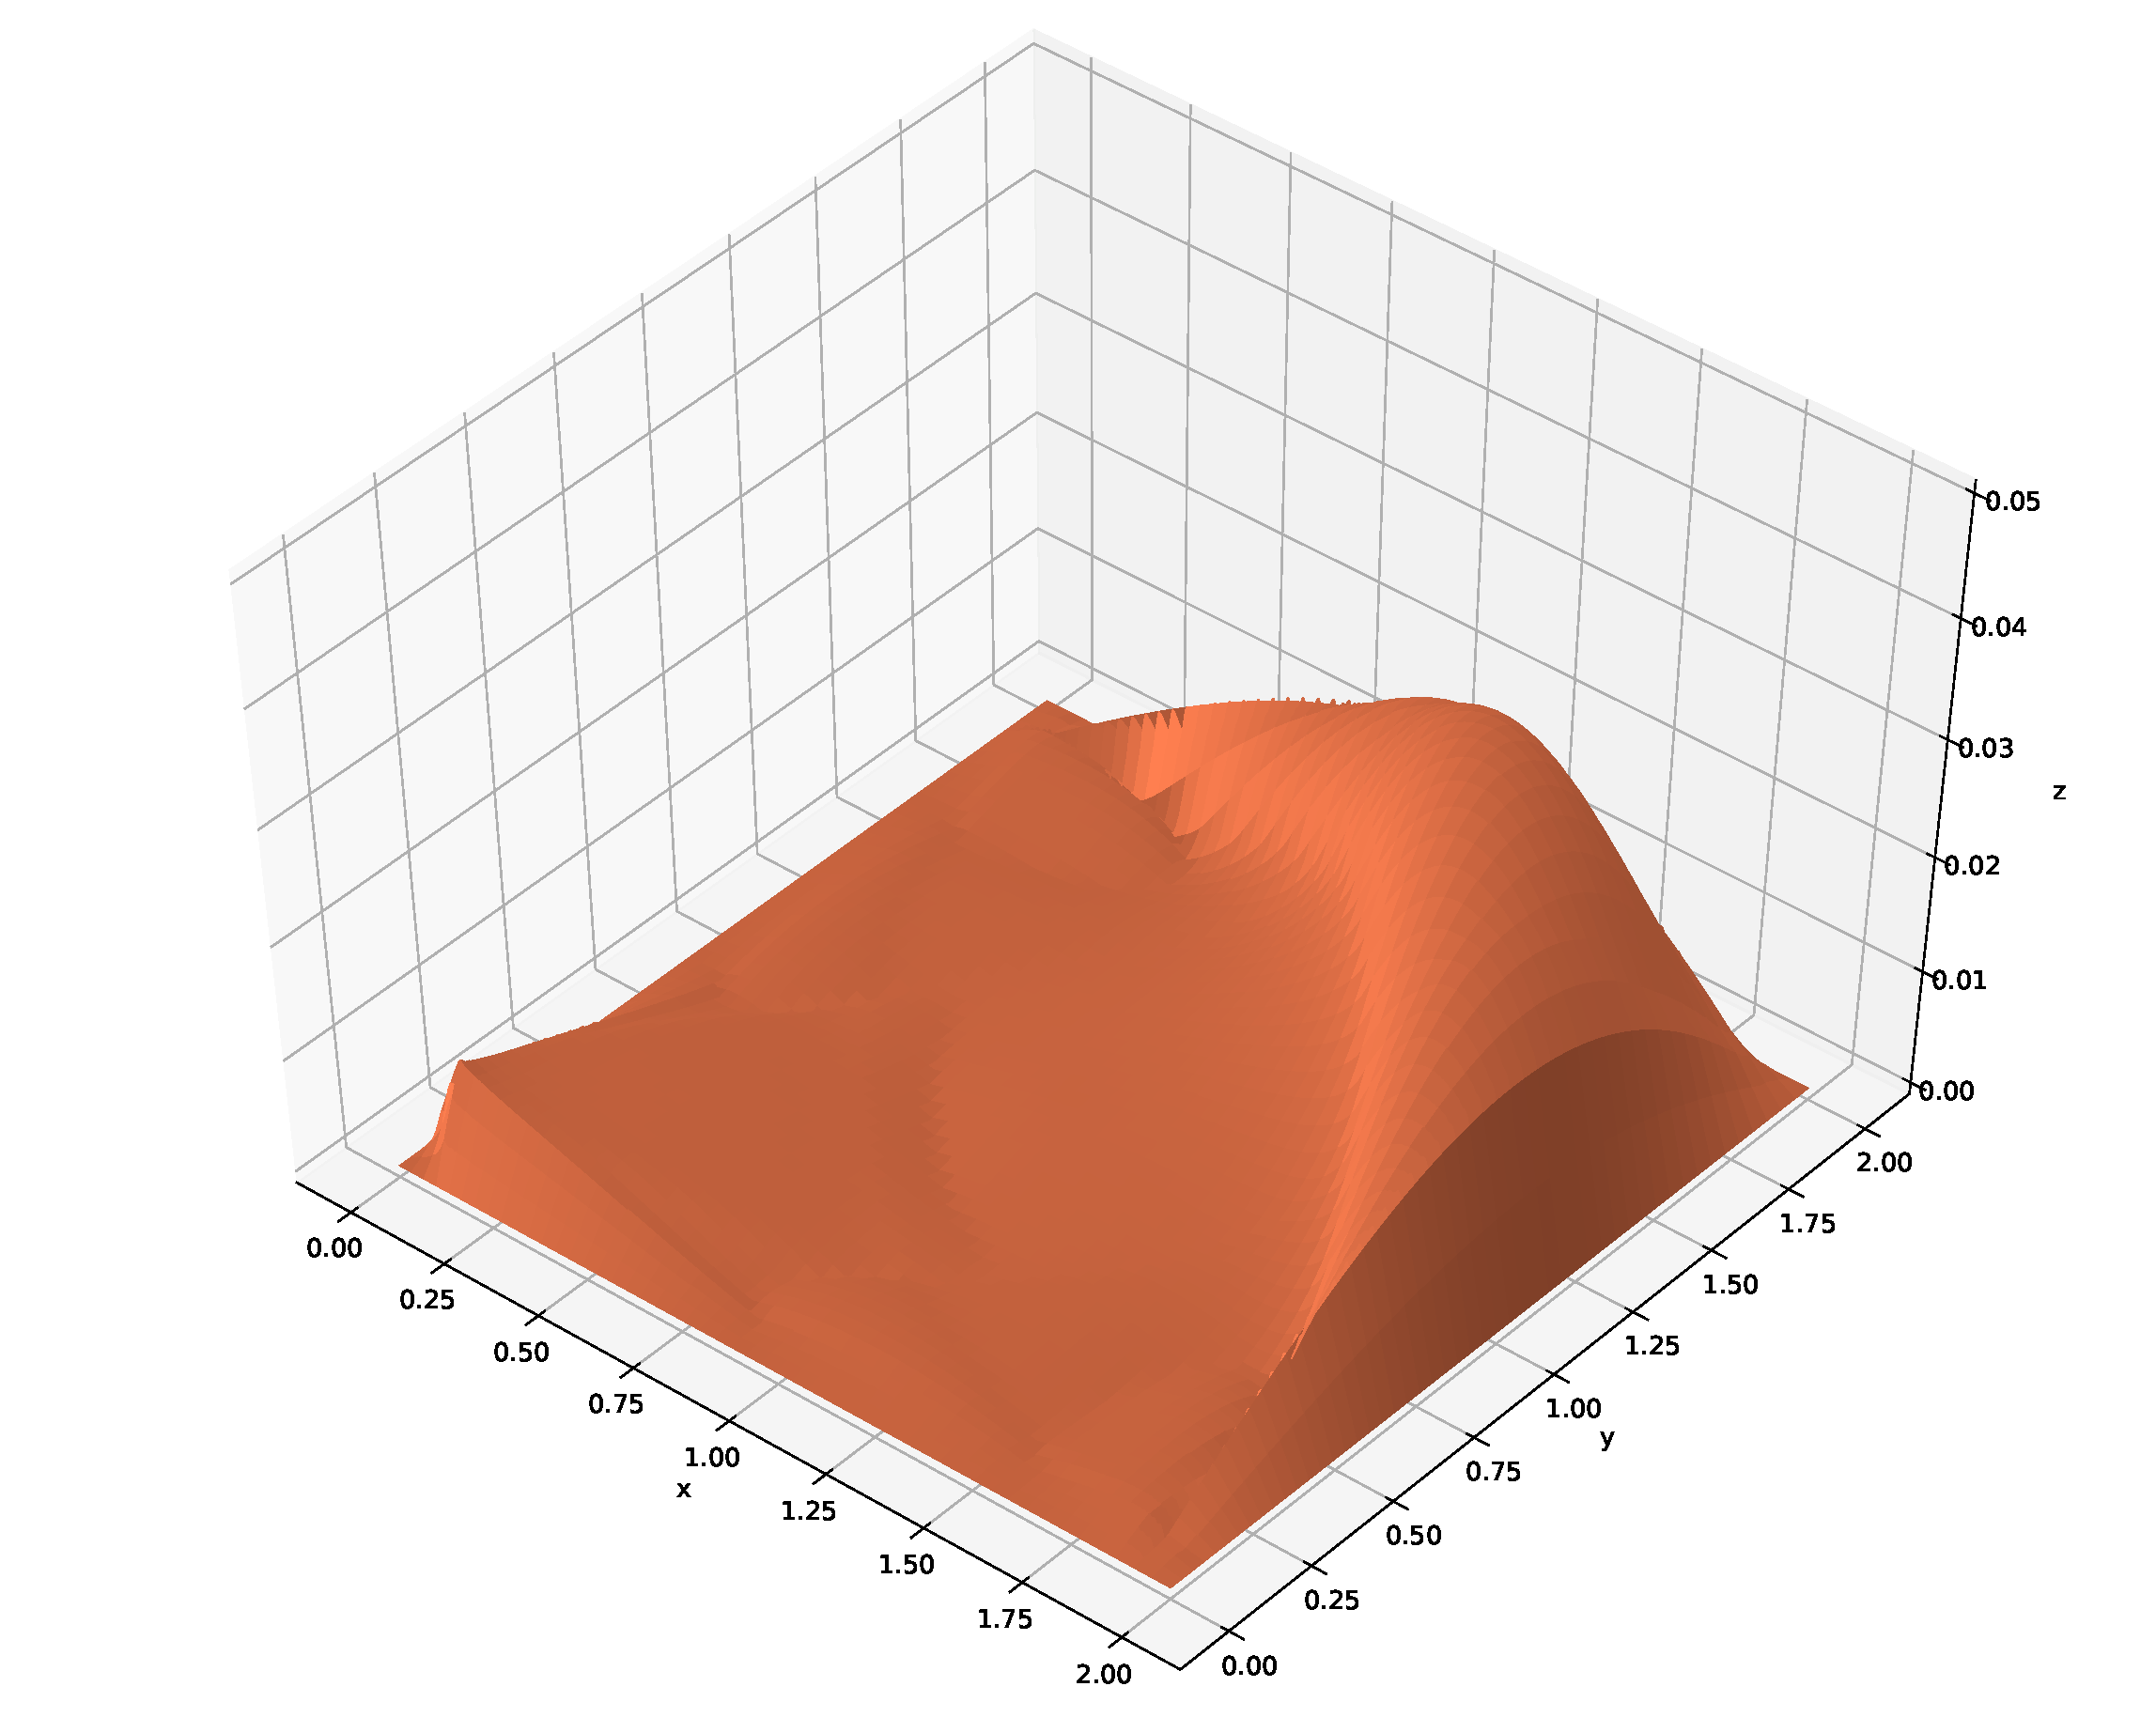
\includegraphics[width=\textwidth]{pics/diff.pdf}
                \caption{В увеличенном масштабе}
                \label{fig:plot_diff_a}
            \end{subfigure}
            \begin{subfigure}[b]{0.49\textwidth}
                \centering
                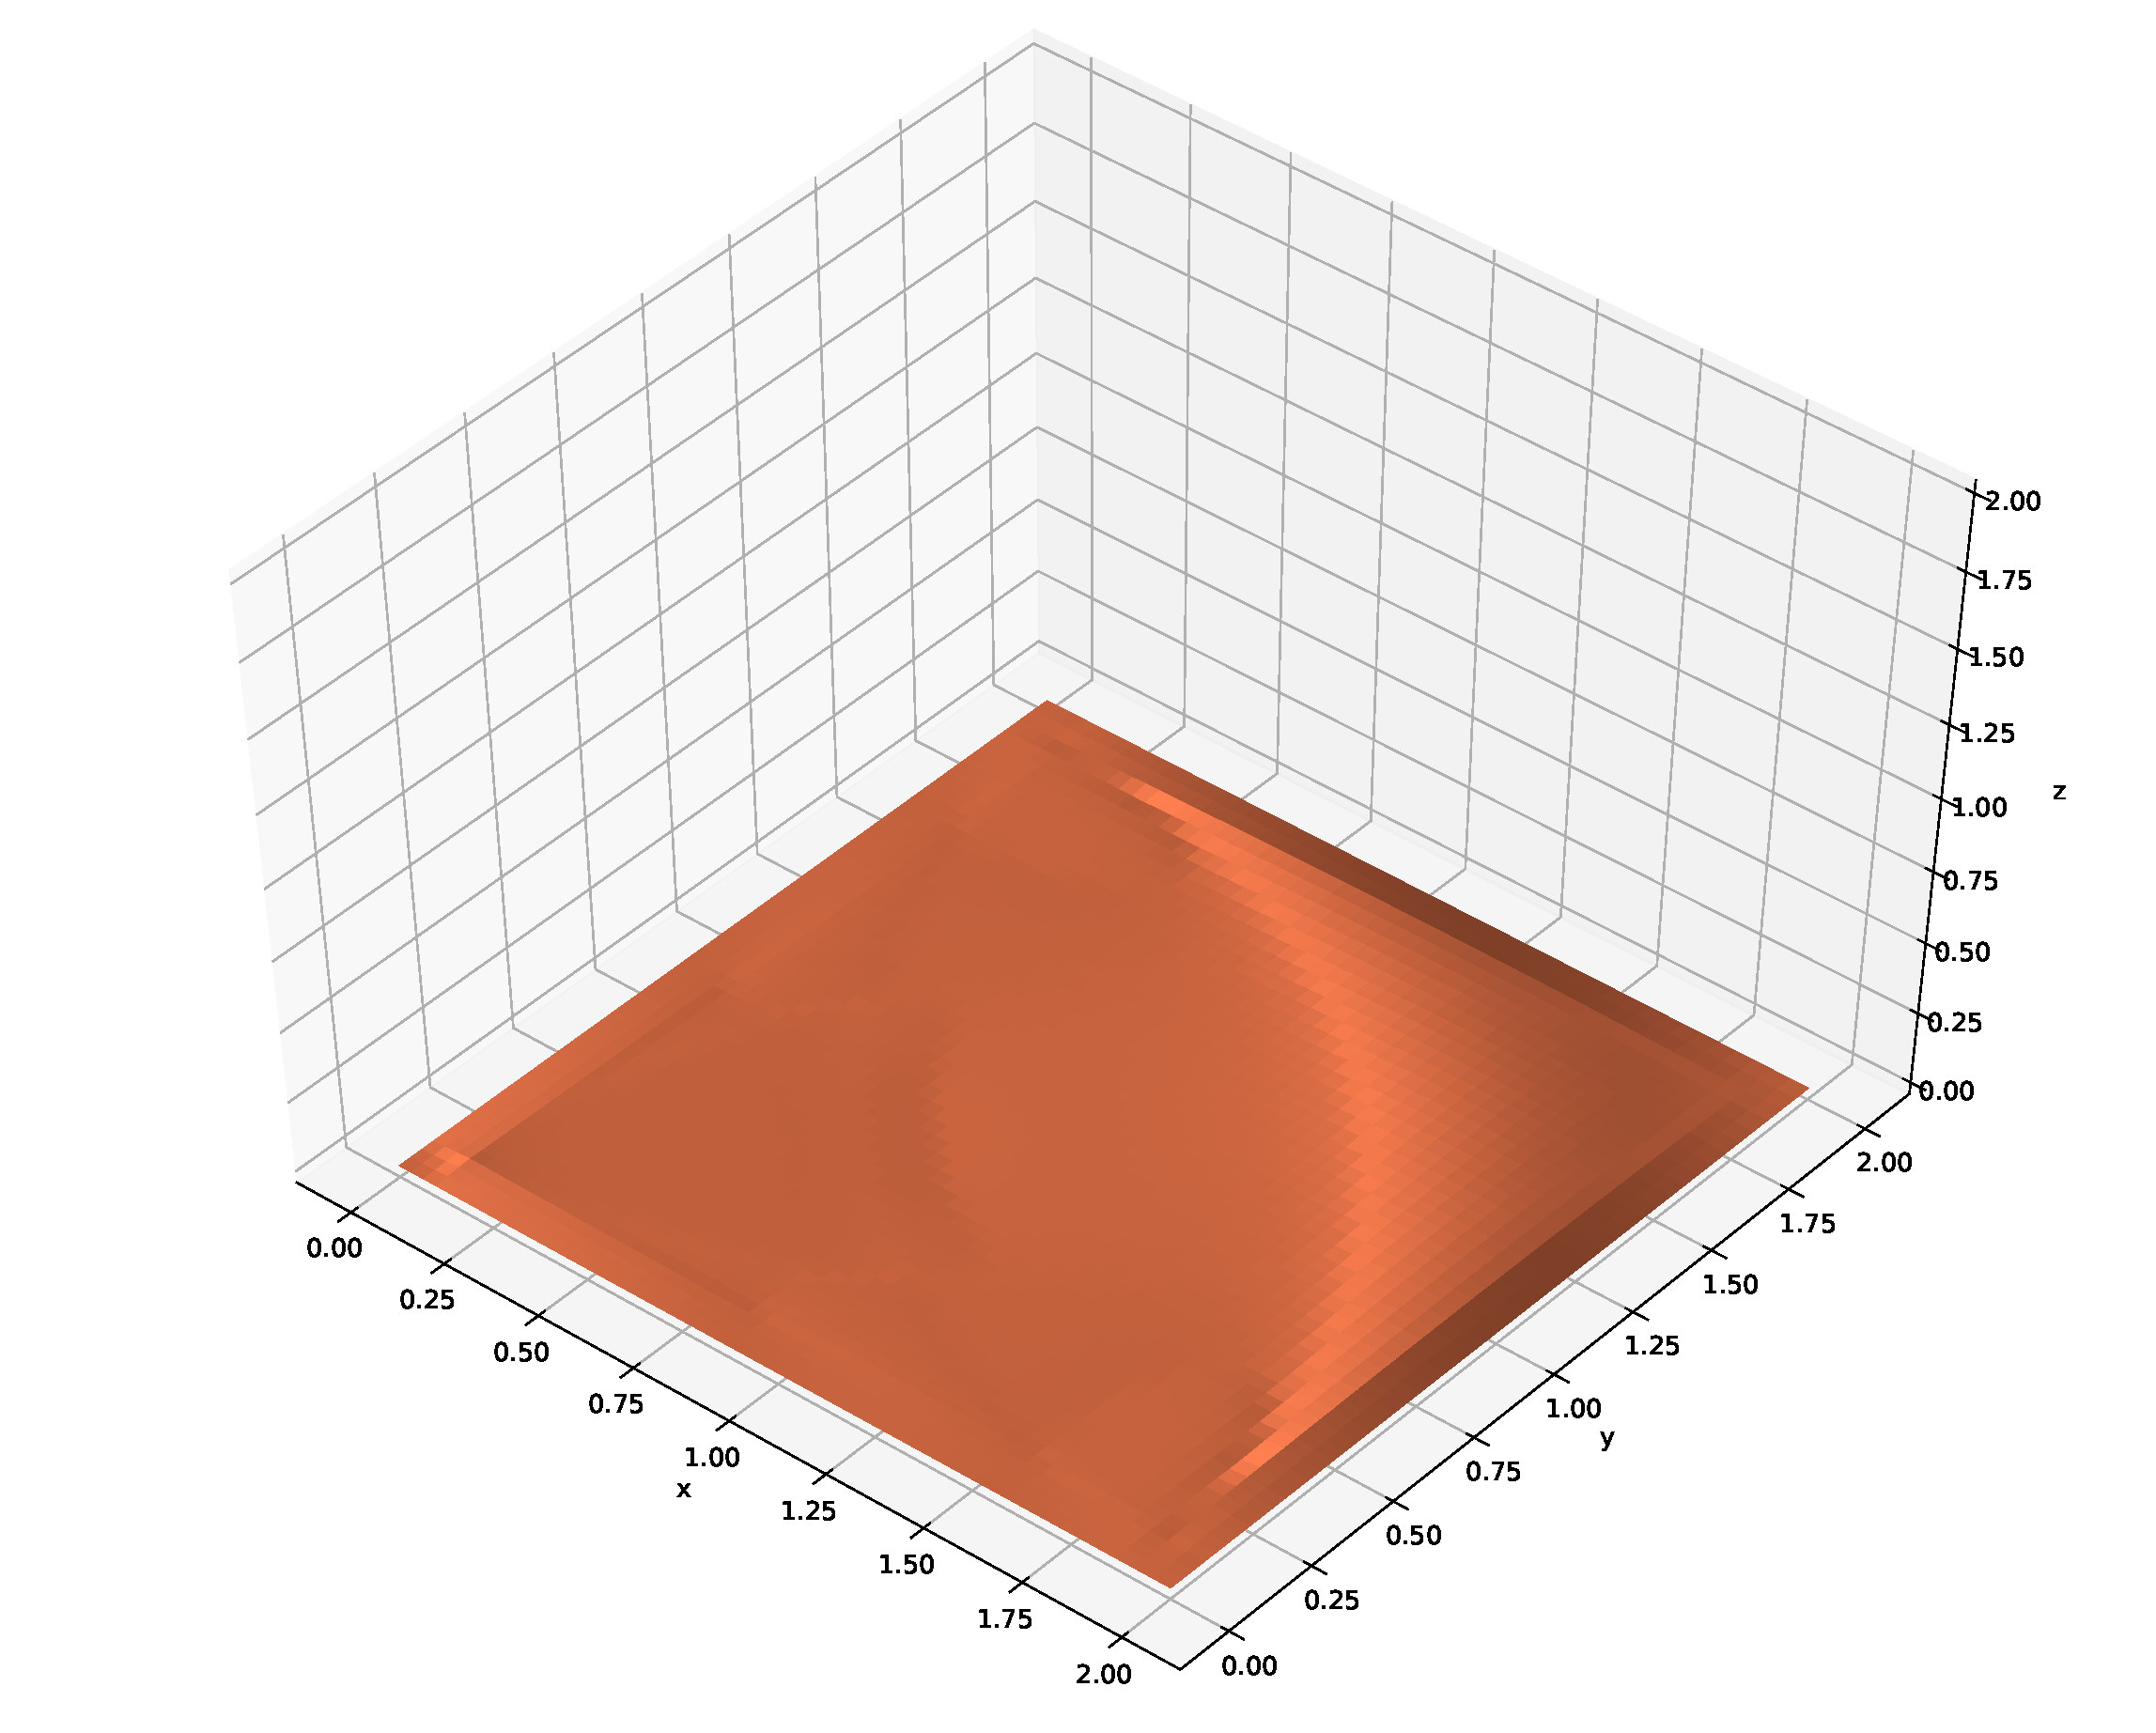
\includegraphics[width=\textwidth]{pics/diff_sc.pdf}
                \caption{{В масштабе решений}}
                \label{fig:plot_diff_b}
            \end{subfigure}
            \caption{Графики разности численного и аналитического решений дифференицальной задачи}
            \label{fig:plot_diff}
        \end{figure}

    \section{Реализация на CUDA}
        CUDA версия программы тестировалась на компьютере <<Ломоносов>> в очереди gputest. Т.к. данная очередь ограничивается максимум 8 узлами, данные были получены только до 16 процессов/видеокарт.

        Ускорением программы называют отношение времени выполнения последовательной версии программы к времени выполнения параллельной:
        $$S = \frac{T_1}{T_p},$$
        где $T_p$ -- время выполнения программы на $p$ процессах.

        Для оценки масштабируемости параллельной программы используется понятие эффективности:
        $$E = \frac{S}{p}$$

        В результате запусков программы для разных количеств процессоров и видеокарт, были получены Таблицы \ref{tab:lom_mpi_low} и \ref{tab:lom_cuda} времени работы программ и их ускорений.

        Ускорение для CUDA версии программы считалось относительно последовательной версии программы, реализованной без использования видеокарт.

        \begin{table}[H]
            \centering
            \caption{MPI версия программы}
            \label{tab:lom_mpi_low}
            \begin{tabular}{llll}
            \rowcolor[HTML]{C0C0C0}
            \textbf{Число процессоров} & \textbf{Число точек сетки}           & \textbf{Время решения, сек} & \textbf{Ускорение} \\
            \rowcolor[HTML]{EFEFEF}
            1                          &                                      & 167.95                      & 1                  \\
            2                          &                                      & 86.12                       & 1.95               \\
            4                          &                                      & 42.66                       & 3.94               \\
            8                          &                                      & 22.09                       & 7.60               \\
            16                         & \multirow{-4}{*}{$1000 \times 1000$} & 10.72                       & 15.67              \\
            \rowcolor[HTML]{EFEFEF}
            1                          &                                      & 676.53                      & 1                  \\
            2                          &                                      & 346.07                      & 1.95               \\
            4                          &                                      & 173.75                      & 3.89               \\
            8                          &                                      & 95.30                       & 7.1                \\
            16                         & \multirow{-4}{*}{$2000 \times 2000$} & 45.49                       & 14.87
            \end{tabular}
        \end{table}

        \begin{table}[H]
            \centering
            \caption{CUDA версия программы}
            \label{tab:lom_cuda}
            \begin{tabular}{llll}
            \rowcolor[HTML]{C0C0C0}
            \textbf{Число видеокарт} & \textbf{Число точек сетки}           & \textbf{Время решения, сек} & \textbf{Ускорение} \\
            \rowcolor[HTML]{EFEFEF}
            1                        &                                      & 101.23                      & 1.66               \\
            2                        &                                      & 59.05                       & 2.84               \\
            4                        &                                      & 31.23                       & 5.38               \\
            8                        &                                      & 18.11                       & 9.27               \\
            16                       & \multirow{-4}{*}{$1000 \times 1000$} & 9.99                        & 16.81              \\
            \rowcolor[HTML]{EFEFEF}
            1                        &                                      & 341.68                      & 1.98               \\
            2                        &                                      & 188.97                      & 3.58               \\
            4                        &                                      & 104.55                      & 6.47               \\
            8                        &                                      & 55.39                       & 12.21              \\
            16                       & \multirow{-4}{*}{$2000 \times 2000$} & 31.70                       & 21.34
            \end{tabular}
        \end{table}

        \subsection{Выводы}
            Для более наглядного анализа таблиц, нарисуем графики ускорений и эффективностей (Рис. \ref{fig:cuda_s} и \ref{fig:cuda_e}). Эффективности програм считались относительно последовательной версии каждого варианта. Таким образом, для CUDA версии эффективность считалась относительно CUDA версии на одной видеокарте, а для MPI версии -- на последовательной версии программы на одном процессоре.

            \begin{figure}[H]
                \centering
                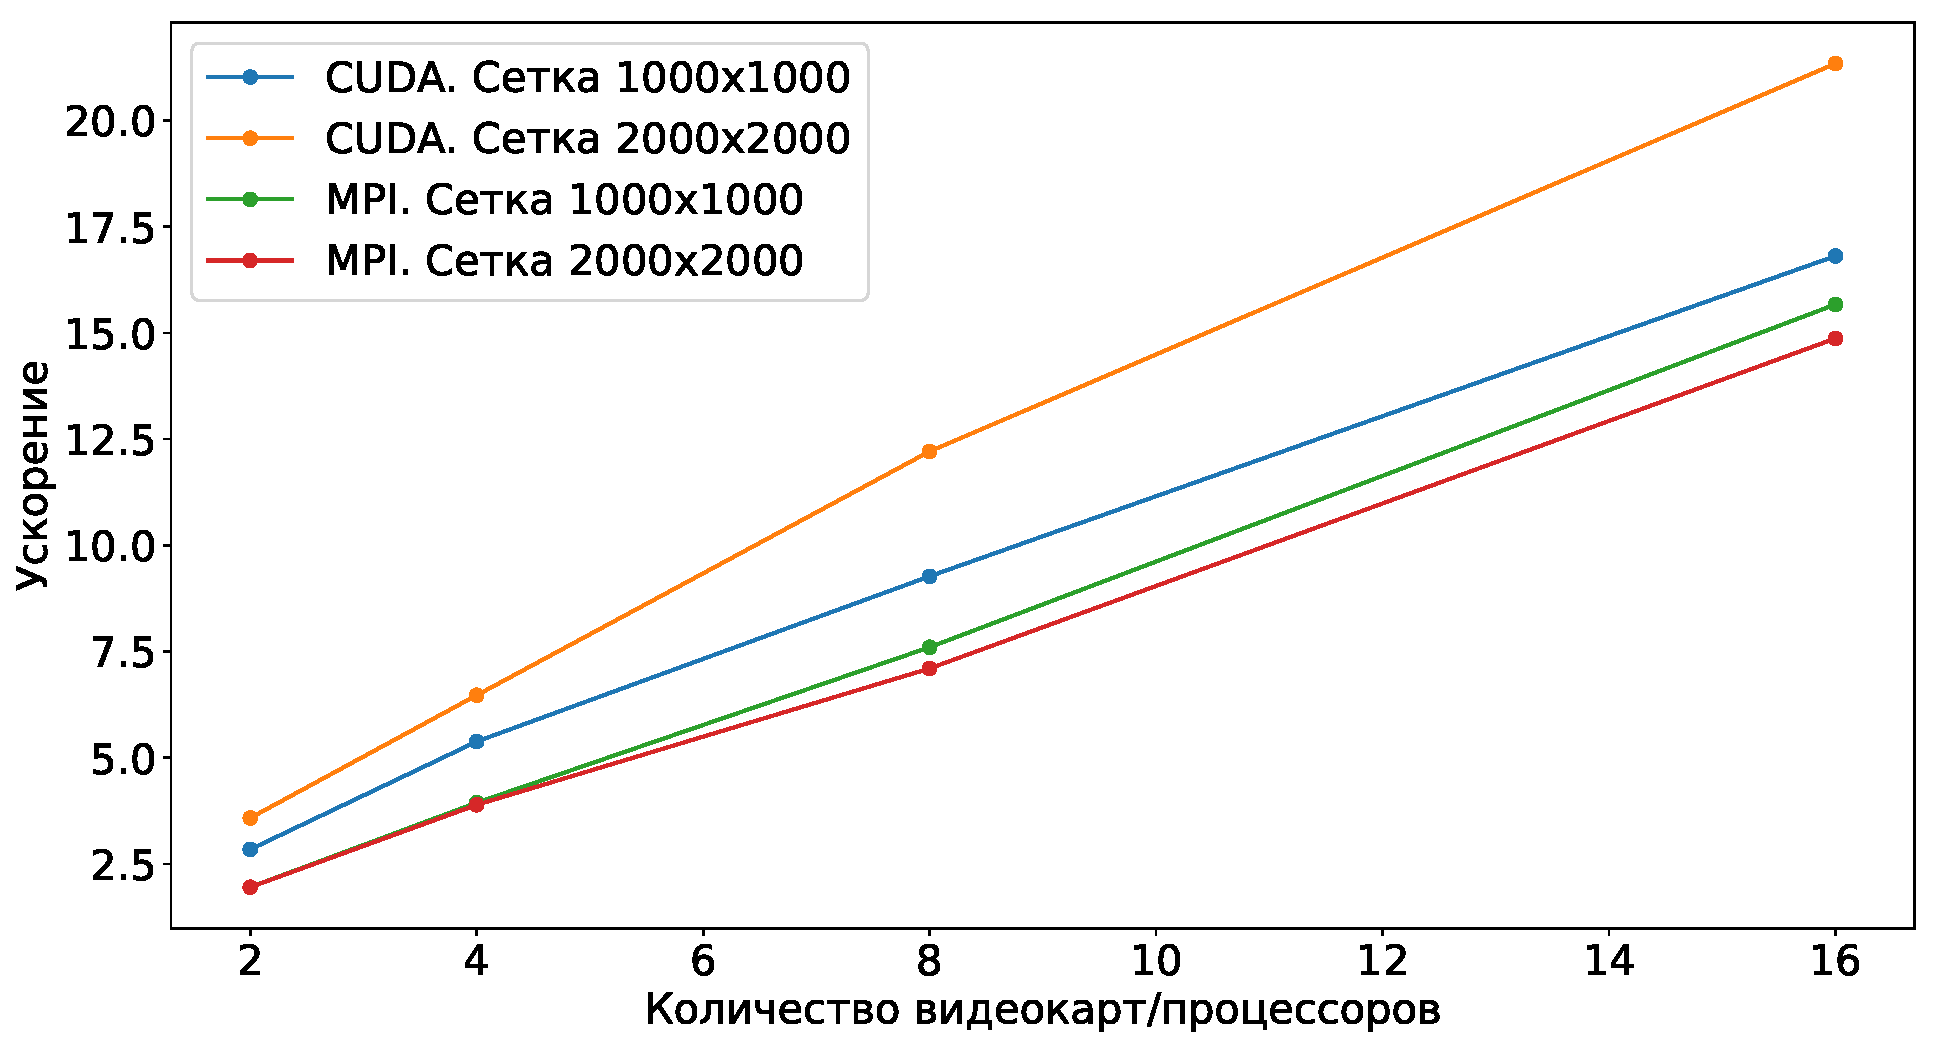
\includegraphics[width=\textwidth]{pics/cuda_s.pdf}
                \caption{Ускорение CUDA и MPI версий}
                \label{fig:cuda_s}
            \end{figure}

            Ускорение CUDA версии (Рис. \ref{fig:cuda_s}) по сравнению с MPI версией на малых размерах сетки не велико, но с ростом размера сетки увеличивается ускорение программы. Данный факт характеризуется особенностью CUDA программ, а именно их ``бутылочным горлышком'' в виде загрузки-выгрузки данных. Чем больше данных и меньше вычилений, тем менее эффективна программа. К тому же, в нашем случае, вычисления на карте растут не линейно с ростом данных, а в 5 раз больше, т.к. идет подсчет оператора Лапласа. Таким образом, чем больше сетка, тем больше данных на видеокарту и тем больше она нагружена, что приводит к большему ускорению.

            \begin{figure}[H]
                \centering
                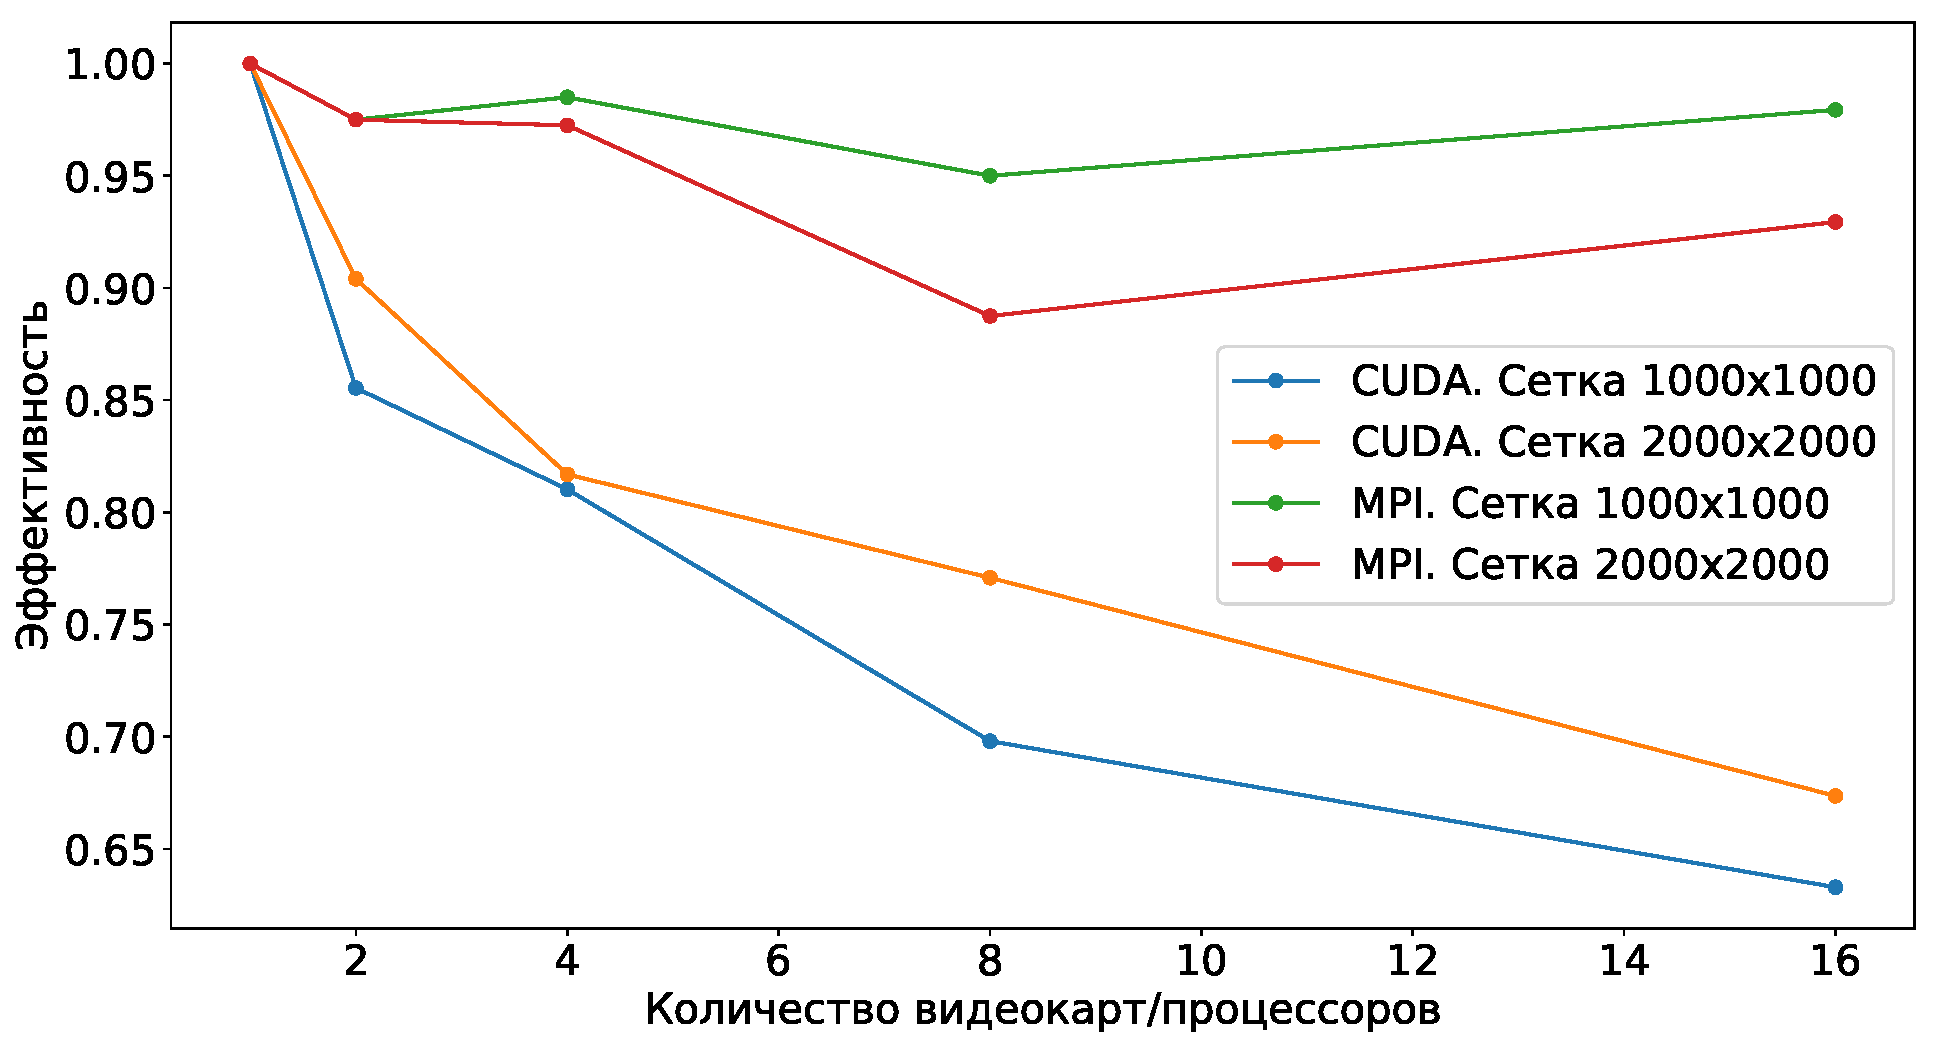
\includegraphics[width=\textwidth]{pics/cuda_e.pdf}
                \caption{Эффективность CUDA и MPI версий}
                \label{fig:cuda_e}
            \end{figure}

            Также по Рис. \ref{fig:cuda_e} эффективности программы можно заметить, что эффективность падает для CUDA программы, но для MPI программы она примерно постоянная. Объясняется это тем, что с увеличением количества видеокарт, данные для обработки одной картой уменьшаются. Это приводит к неполной нагруженности видеокарты. Также при обмене данными между процессами, данные с видеокарты полностью выгружаются, а затем загружаются обратно, что очень затратно при больших количествах данных и процессов. Таким образом, в данной реализации, масштабируемость программы маленькая. Чтобы масштабируемость была хорошей, данные и вычисления должны быть такими, чтобы полностью нагружать видеокарты.

            В дополнение стоит отметить, что корректность программы проверялась также, как и в случае с MPI версией -- невязкой численного решения и аналитического. Также количество итераций и ошибка каждого шага были одинаковы без учета машинной точности, что подтверждает правильность CUDA программы.

    \section{Приложение}\label{sec:appdx}
        Для всех приведенных ниже таблиц время выполнения на одном процессоре для сетки $2000 \times 2000$ было выведено примерными рассчетами. Они указаны через знак $\sim$.
        \begin{table}[H]
            \centering
            \caption{MPI версия программы до схождения на BlueGene/P}
            \label{tab:bg_mpi_full}
            \begin{tabular}{llll}
            \rowcolor[HTML]{C0C0C0}
            \textbf{Число процессоров} & \textbf{Число точек сетки}                   & \textbf{Время решения, сек} & \textbf{Ускорение} \\
            \rowcolor[HTML]{EFEFEF}
            1                          & \multicolumn{1}{c}{\cellcolor[HTML]{EFEFEF}} & 3107.29                     & 1                  \\
            64                         &                                              & 49.79                       & 62.41              \\
            128                        &                                              & 26.67                       & 116.51             \\
            256                        &                                              & 13.91                       & 223.39             \\
            512                        & \multirow{-4}{*}{1000 $\times$ 1000}         & 7.94                        & 391.35             \\
            \rowcolor[HTML]{EFEFEF}
            1                          &                                              & $\sim$23615.39              & 1                  \\
            64                         &                                              & 368.69                      & 64.05              \\
            128                        &                                              & 189.29                      & 124.76             \\
            256                        &                                              & 95.87                       & 246.33             \\
            512                        & \multirow{-4}{*}{2000 $\times$ 2000}         & 51.45                       & 459.00
            \end{tabular}
        \end{table}

        \begin{table}[H]
            \centering
            \caption{MPI+OpenMP версия программы до схождения на BlueGene/P}
            \label{tab:bg_omp_full}
            \begin{tabular}{llll}
            \rowcolor[HTML]{C0C0C0}
            \textbf{Число процессоров} & \textbf{Число точек сетки}                   & \textbf{Время решения, сек} & \textbf{Ускорение} \\
            \rowcolor[HTML]{EFEFEF}
            1                          & \multicolumn{1}{c}{\cellcolor[HTML]{EFEFEF}} & 1085.00                     & 2.86               \\
            64                         &                                              & 19.31                       & 160.92             \\
            128                        &                                              & 11.38                       & 273.05             \\
            256                        &                                              & 6.68                        & 465.16             \\
            512                        & \multirow{-4}{*}{1000 $\times$ 1000}         & 4.47                        & 695.14             \\
            \rowcolor[HTML]{EFEFEF}
            1                          &                                              & $\sim$8137.5                & 2.90               \\
            64                         &                                              & 133.18                      & 177.32             \\
            128                        &                                              & 71.09                       & 332.19             \\
            256                        &                                              & 37.26                       & 633.80             \\
            512                        & \multirow{-4}{*}{2000 $\times$ 2000}         & 21.94                       & 1076.36
            \end{tabular}
        \end{table}

        \begin{table}[H]
            \centering
            \caption{MPI версия программы до схождения на Ломоносов}
            \label{tab:lom_mpi_full}
            \begin{tabular}{llll}
            \rowcolor[HTML]{C0C0C0}
            \textbf{Число процессоров} & \textbf{Число точек сетки}                   & \textbf{Время решения, сек} & \textbf{Ускорение} \\
            \rowcolor[HTML]{EFEFEF}
            1                 &                                      & 473.59             & 1         \\
            8                 &                                      & 66.18              & 7.16      \\
            16                &                                      & 30.34              & 15.61     \\
            32                &                                      & 14.89              & 31.81     \\
            64                &                                      & 7.52               & 62.98     \\
            128               & \multirow{-5}{*}{1000 $\times$ 1000} & 4.54               & 104.31    \\
            \rowcolor[HTML]{EFEFEF}
            1                 &                                      & $\sim$3820.60      & 1         \\
            8                 &                                      & 523.37             & 7.3       \\
            16                &                                      & 254.14             & 15.03     \\
            32                &                                      & 126.12             & 30.29     \\
            64                &                                      & 58.61              & 65.19     \\
            128               & \multirow{-5}{*}{2000 $\times$ 2000} & 29.92              & 127.69
            \end{tabular}
        \end{table}


\end{document}
